%\documentclass[12pt,letterpaper]{article}
\documentclass[12pt]{amsart}

\usepackage[left=1in, right=1in, top=.5in, bottom=.5in]{geometry}
\usepackage{latexsym,amssymb,amsmath,amsthm,amsopn,verbatim, mathpazo, graphicx, lmodern, hyperref, color}
%\usepackage{latexsym,amssymb,amsmath,amsthm,amsopn,verbatim, mathpazo, graphicx}
\newcommand{\vs}{\vskip.5cm}
\newcommand{\hs}{\hskip1cm}
\newcommand{\ds}{\displaystyle}
\setlength{\parindent}{0pt}


\usepackage[T1]{fontenc}
\usepackage{libertine}
\renewcommand*\familydefault{\sfdefault}  %% Only if the base font of the document is to be sans serif


\newtheorem{theorem}{Theorem}[section]
\newtheorem{corollary}{Corollary}[theorem]
\newtheorem{lemma}[theorem]{Lemma}
\newtheorem{definition}[theorem]{Definition}
\newtheorem{example}[theorem]{Example}

\newcommand\indep{\protect\mathpalette{\protect\independenT}{\perp}}
\def\independenT#1#2{\mathrel{\rlap{$#1#2$}\mkern2mu{#1#2}}}

\begin{document}


%----------------------------------------------------------------------------
\setcounter{section}{3}
%\setcounter{subsection}{1}
%\setcounter{theorem}{1}
Day 6 BSTA 511/611
{\huge  
\section*{Chapter 3: Distributions of Random Variables (Part 1)}
}

%----------------------------------------------------------------------------


%----------------------------------------------------------------------------
{\large 
%----------------------------------------------------------------------------

\emph{Day 6 topics}:

Section 3.1: Random variables  \newline
Section 3.2: Binomial distribution

\hrulefill
%----------------------------------------------------------------------------
%\begin{example}  \textbf{text.} \newline
%
%\begin{enumerate}
%\item 
%
%\vspace{2cm}
%
%\item 
%
%\vspace{2cm}
%
%\item 
%
%\vspace{2cm}
%\end{enumerate}
%\end{example} 

%\newpage
%----------------------------------------------------------------------------

%Section 3.1
\subsection{Random variables}

\begin{definition} A \textbf{random variable (r.v.)} assigns numerical values to the outcome of a random phenomenon.
\end{definition}

Notation: \newline 
A random variable is usually denoted with a capital letter such as $X$, $Y$, or $Z$.

\vspace{1cm}
%----------------------------------------------------------------------------
\begin{example}  \textbf{Data points} \newline
Suppose you have a dataset of size 3 ($n=3$) with $x_1 = 5, x_2 = 3,$ and $x_3 = 6$. 
\begin{itemize}
\item Each data point is the outcome of a random phenomenon

\item Each data point is a numerical value
\item The data points are examples of values of a sequence of random variables $X_1, X_2,$ and $X_3$
\item For datasets, we almost always assume the data points came from random variables that are independent and have the same \textbf{distribution}. 
\item To calculate the likelihood of data, we need to know the distribution of the random variable that models the data.

\item First, let's remind ourselves how to calculate them mean and variance of a dataset:
	\begin{itemize}
	\item What is the mean of the data points?

\vspace{2cm}
	\item What are the variance and standard deviation of the data points?


	\end{itemize}


\end{itemize}
\end{example} 

\newpage
%----------------------------------------------------------------------------

%3.1.1
%\subsubsection{Distributions of random variables}


%----------------------------------------------------------------------------
\begin{example}  \textbf{Rolling a die} \newline
Suppose you roll a fair die. Let the random variable (r.v.) $X$ be the outcome of the roll, i.e. the value of the face showing on the die. 

\begin{enumerate}
\item What is the probability distribution of the r.v. $X$?
\vspace{3cm}

\item  What is the expected outcome of the r.v. $X$?



\vspace{5cm}

\item Now suppose the 6-sided die is not fair. How would we calculate the expected outcome?

%undelete
\vspace{1cm}
\begin{tabular}{| c | c |}
  \hline                       
  x & $\mathbb{P}(X=x)$  \\
   \hline     
  1 & 0.10 \\
  2 & 0.20  \\
  3 & 0.05  \\
  4 & 0.05  \\
  5 & 0.25  \\
  6 & 0.35  \\
  \hline  
\end{tabular}

%
%%delete
%\color{blue}
%\vspace{1cm}
%\begin{tabular}{| c | c | c |}
%  \hline                       
%  $x$ & $\mathbb{P}(X=x)$ & $x\mathbb{P}(X=x)$ \\
%   \hline     
%  1 & 0.10 & 0.1\\
%  2 & 0.20  & 0.4\\
%  3 & 0.05  & 0.15\\
%  4 & 0.05  & 0.2\\
%  5 & 0.25  & 1.25\\
%  6 & 0.35  & 2.10\\
%   \hline   
%   sum & 1 & $\mu = 4.2$ \\
%  \hline  
%\end{tabular}
%\color{black}
%%delete

\vspace{2cm}
\end{enumerate}
\end{example} 

\newpage
%----------------------------------------------------------------------------


(From Textbook $\S$ 2.1.5)
\begin{definition} A \textbf{probability distribution} consists of all disjoint outcomes and their associated probabilities.
\end{definition}

\textbf{Rules for a probability distribution} \newline
A probability distribution is a list of all possible outcomes and their associated probabilities that satisfies three rules: 
\begin{enumerate}
\setlength{\itemsep}{0mm}
\item The outcomes listed must be disjoint.
\item Each probability must be between 0 and 1.
\item The probabilities must total to 1. \vspace{1mm}
\end{enumerate}

\vspace{0.5cm}

Probability distributions are usually either \textbf{discrete} or \textbf{continuous}, depending on whether the random variable is discrete or continuous.

\vspace{1cm}

(Back to Textbook $\S$ 3.1.1)
\begin{definition} A \textbf{discrete} r.v. $X$ takes on a finite number of values or countably infinite number of possible values.
\end{definition}

\begin{definition} A \textbf{continuous} r.v. $X$ can take on any real value in an interval of values or unions of intervals.\end{definition}


\vspace{2cm}

\newpage
%----------------------------------------------------------------------------

$\S$ \textbf{3.1.2 Expectation}

\vspace{.5cm}

\begin{itemize}
\item We call the mean of a random variable its \textbf{expected value}
\item The expected value is calculated as a weighted average
\end{itemize}

\vspace{.5cm}

\begin{definition}{\textbf{Expected value} of a discrete random variable} \newline
If $X$ takes on outcomes $x_1$, ..., $x_k$ with probabilities $P(X=x_1)$, ..., $P(X=x_k)$, the expected value of $X$ is the sum of each outcome multiplied by its corresponding probability:

%%delete
%\color{blue}
%\begin{align}
%\mu = E(X) 	&= x_1 P(X=x_1) + \cdots + x_k P(X=x_k) \notag \\
%&= \sum_{i=1}^{k}x_iP(X=x_i). \notag 
%\end{align}
%\color{black}

\vspace{3cm}

\end{definition}



$\S$ \textbf{3.1.3 Variability of random variables}

\vspace{.5cm}

\begin{itemize}
\item Just like with data, the variability of a r.v. is described with its variance or standard deviation.
\item Squared deviations from the mean are weighted by their respective probabilities
\end{itemize}

\vspace{.5cm}

\begin{definition}{\textbf{Variance} of a discrete random variable} \newline
If $X$ takes on outcomes $x_1$, ..., $x_k$ with probabilities $P(X=x_1)$, \dots, $P(X=x_k)$ and expected value $\mu=E(X)$, then the variance of $X$, denoted by $\text{Var}(X)$ or $\sigma^2$, is

%%delete
%\color{blue}
%\begin{align}
%Var(X) &= (x_1-\mu)^2 P(X=x_1) + \cdots \notag + (x_k-\mu)^2 P(X=x_k) \notag \\
%&= \sum_{i=1}^{k} (x_i - \mu)^2 P(X=x_i). \notag 
%\end{align}
%
%\color{black}
\vspace{4.5cm}
\end{definition}

\begin{definition}{\textbf{Standard deviation} of a discrete random variable} \newline
The standard deviation of $X$, labeled $SD(X)$ or $\sigma$, is 

%%delete
%\color{blue}
%$$ SD(X) = \sigma = \sqrt{\sigma^2}$$
%\color{black}

\end{definition}



\newpage
%----------------------------------------------------------------------------
\begin{example}  \textbf{Rolling a fair die: variance} \newline
Suppose you roll a fair 6-sided die. Let the random variable (r.v.) $X$ be the outcome of the roll, i.e. the value of the face showing on the die.  \newline
Find the variance and standard deviation of $X$.


%undelete
\vspace{1cm}
\begin{tabular}{| c | c |}
  \hline                       
  x & $\mathbb{P}(X=x)$  \\
   \hline     
      &  \\
  1 & 1/6 \\
     &  \\
  2 & 1/6  \\
      &  \\
  3 & 1/6  \\
      &  \\
  4 & 1/6  \\
      &  \\
  5 & 1/6  \\
      &  \\
  6 & 1/6  \\
      &  \\
  \hline  
\end{tabular}

%%delete
%\vspace{1cm}
%
%\color{blue}
%
%$$\mu = 3.5$$
%
%\vspace{1cm}
%\begin{tabular}{| c | c | c | c | c |}
%  \hline                       
%  $x$ & $\mathbb{P}(X=x)$ &  $x - \mu$ & $(x - \mu)^2$\\
%   \hline     
%  1 & 1/6  & -2.5 &  6.25\\
%  2 & 1/6    & -1.5 & 2.25 \\
%  3 & 1/6    & -0.5 &  0.25\\
%  4 & 1/6    & 0.5 & 0.25 \\
%  5 & 1/6   & 1.5   &  2.25\\
%  6 & 1/6    &2.5 & 6.25\\
%   \hline   
%   sum & 1 &    &  $\sigma^2 = 17.5$\\
%  \hline  
%\end{tabular}
%\vspace{2cm}
%%delete
%$$\sigma =4.1833 $$




\end{example} 



 \newpage
%----------------------------------------------------------------------------

%----------------------------------------------------------------------------
\begin{example}  \textbf{Vaccinated people testing positive for Covid-19} \newline
About 25\% of people that test positive for Covid-19 are vaccinated for Covid-19.\newline
Define the r.v. $X$ to be 1 if someone that tests positive is vaccinated and 0 if they are not vaccinated.


\begin{enumerate}
\item Make a table for the probability distribution for the r.v. $X$

\vspace{3cm}

\item What is the expected value of $X$?

\vspace{5cm}
%%delete
%\color{blue}
%$$\mathbb{E}[X] = p = 0.25$$
%\color{black}

\item What is the variance of $X$?

\vspace{2cm}
%%delete
%\color{blue}
%$$Var[X] = pq = 0.25\cdot0.75 = 0.1875$$
%$$SD[X] = 0.4330127$$
%
%\color{black}
\end{enumerate}

%\vspace{1cm}

%\vspace{1cm}
\end{example} 





\newpage
%----------------------------------------------------------------------------


$\S$ \textbf{3.1.4 Linear combinations of random variables}

\vspace{1cm}
%%delete
%\color{blue}
%Seems abstract, but actually fundamental to basic statistical theory - using it all the time!
%\color{black}

%----------------------------------------------------------------------------
%\vspace{.5cm}

\begin{definition}{\textbf{Linear combinations} of random variables.} \newline
If $X$ and $Y$ are random variables and $a$ and $b$ are constants, then 
%%delete
%\color{blue}
%$$aX+bY$$
%\color{black}
\vspace{2cm}

is a linear combination of the random variables.
\end{definition}


%\vspace{1.5cm}

%----------------------------------------------------------------------------
\begin{theorem}{\textbf{Expected value of a linear combination} of random variables.} \newline
If $X$ and $Y$ are random variables and $a$ and $b$ are constants, then 
%%delete
%\color{blue}
%$$\mathbb{E}(aX + bY) = a\mathbb{E}(X) + b\mathbb{E}(Y) = a\mu_X + b\mu_Y$$
%\color{black}
\vspace{3cm}


\end{theorem}



%%----------------------------------------------------------------------------
%\begin{example}  \textbf{Rolling 3 dice} \newline
%Suppose you roll 3 fair 6-sided dice.  \newline
%Let the random variables $X_1, X_2, X_3$ be the values shown on the 3 dice.  \newline
%What is the expected sum of the 3 dice?
%
%\vspace{1cm}
%
%%delete
%\color{blue}
%
%\color{black}
%
%\vspace{1cm}
%\end{example} 



%----------------------------------------------------------------------------
\begin{example}  \textbf{Expected money for rolling 3 dice} \newline
Let the random variables $X_1, X_2, X_3$ be the values shown on 3 fair 6-sided dice rolls. \newline 
Suppose you are given in dollars the amount of the first roll, plus twice the value of the second roll, plus 4 times the value of the third roll. \newline 
How much money do you expect to get?  \newline 
%What is the standard deviation of the amount?

%\vspace{1cm}

%%delete
%\color{blue}
%$$\mathbb{E}(X_1 + 2X_2 + 4X_3) = \mathbb{E}(X_1) + 2\mathbb{E}(X_2) + 4\mathbb{E}(X_3) = 7\cdot 3.5 = 24.5$$
%\color{black}

\end{example} 

\vspace{2cm}

%%delete
%\color{blue}
%Expected value of the sample mean
%\color{black}


\newpage
%----------------------------------------------------------------------------

Make sure to correct typo in textbook!!!

\vspace{2cm}

\begin{figure}[h!]
  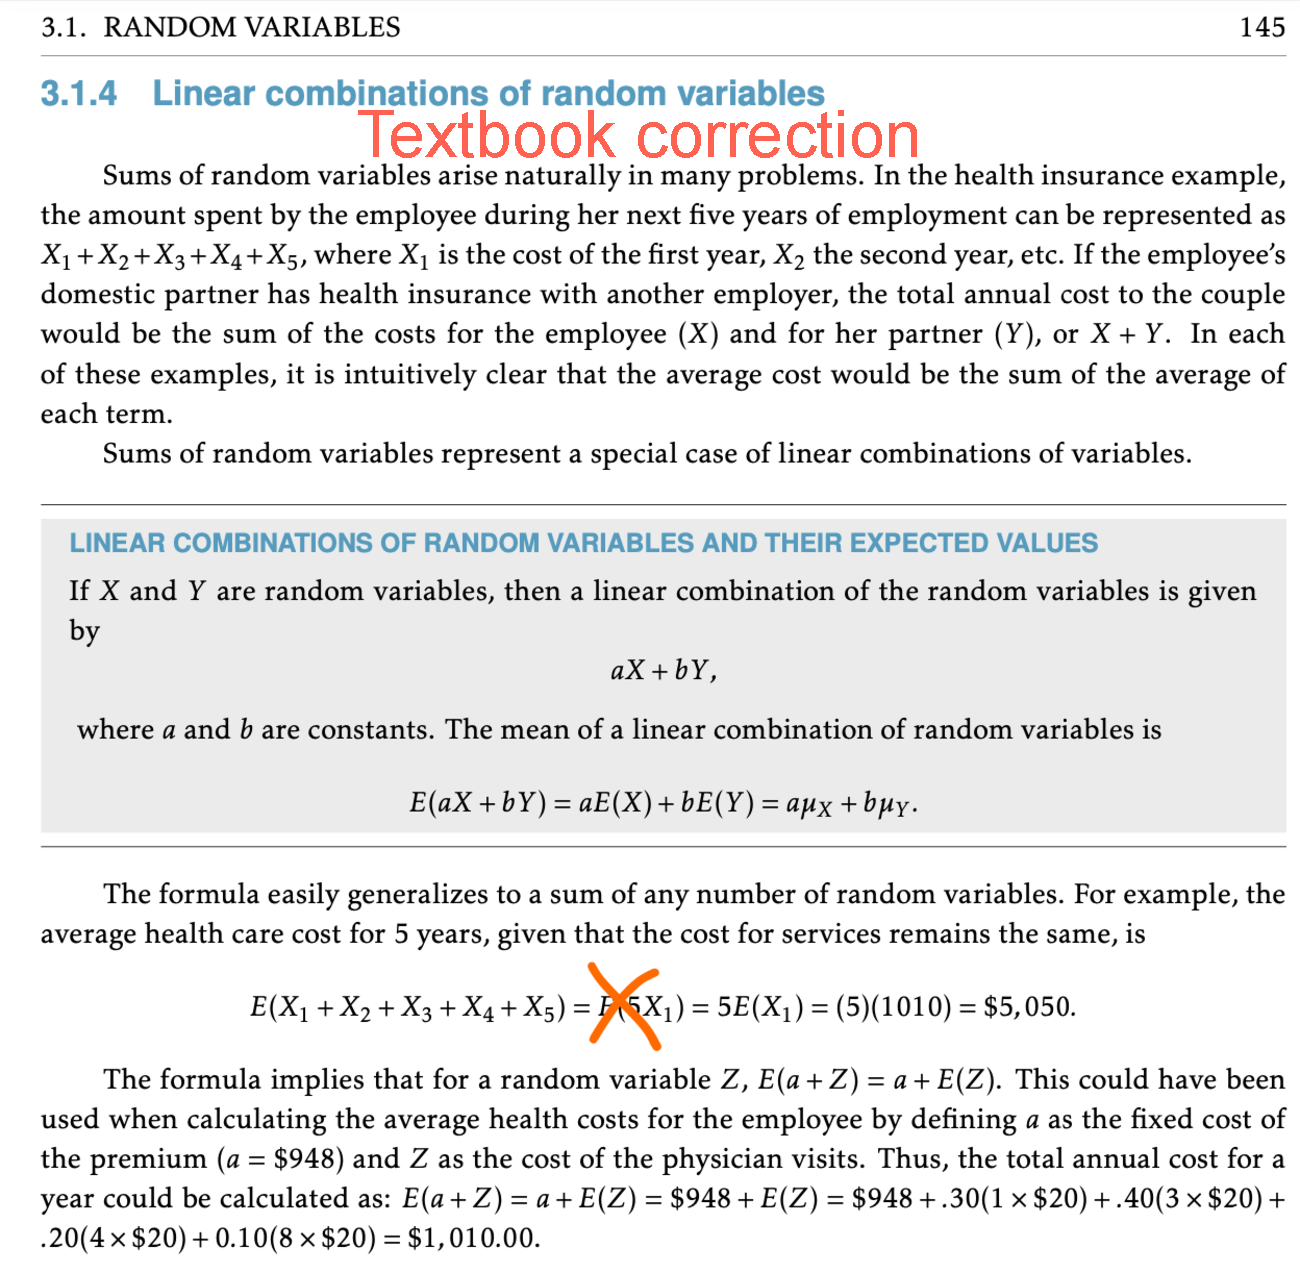
\includegraphics[width=7in]{img/VH_LinearCombo_E[5X]_error.pdf}
  %\caption{Normal (Gaussian) distribution}
  \label{fig:BookError}
\end{figure}



\newpage
%----------------------------------------------------------------------------
\begin{theorem}{\textbf{Variance of a linear combination} of random variables.} \newline
If $X$ and $Y$ are INDEPENDENT random variables and $a$ and $b$ are constants, then 
%%delete
%\color{blue}
%$$\text{Var}(aX + bY) = a^2 \text{Var}(X) + b^2\text{Var}(Y)$$
%\color{black}
\vspace{3.5cm}


\end{theorem}

%----------------------------------------------------------------------------
\begin{example}  \textbf{Variance of money for rolling 3 dice} \newline
Let the random variables $X_1, X_2, X_3$ be the values shown on 3 fair 6-sided dice rolls. \newline 
Suppose you are given in dollars the amount of the first roll, plus twice the value of the second roll, plus 4 times the value of the third roll. \newline 
What are the variance and standard deviation of the amount you get from the 3 rolls?  \newline 


%\vspace{1cm}

%%delete
%\color{blue}
%$$\text{Var}(X_1 + 2X_2 + 4X_3) = \text{Var}(X_1) + 4\text{Var}(X_2) + 16\text{Var}(X_3) = 21\cdot 17.5 = 367.5$$
%\vspace{1cm}
%$$\text{SD}(X_1 + 2X_2 + 4X_3) = \sqrt{367.5} =19.17029 $$
%\color{black}
%%\vspace{1cm}
\end{example} 



%%delete
%\vspace{1cm}
%\color{blue}
%Variance of the sample mean
%\color{black}


 \newpage
%----------------------------------------------------------------------------

%----------------------------------------------------------------------------
\begin{example}\label{VaccBinom}  \textbf{Vaccinated people testing positive for Covid-19 (revisited)} \newline
About 25\% of people that test positive for Covid-19 are vaccinated for Covid-19.\newline
Define the r.v. $X_i$ to be 1 if someone that tests positive is vaccinated and 0 if they are not vaccinated. \newline
Suppose 3 people have tested positive for Covid-19 (independently of each other). \newline
Let $T$ denote the number of people that are vaccinated amongst the 3 that tested positive.


\begin{enumerate}
\item Using the r.v.'s $X_i$, write a mathematical equation for calculating $T$.

\vspace{2cm}
%%delete
%\color{blue}
%$$T = \sum_{i=1}^3 X_i$$
%\color{black}

\item What is the expected value of $T$?

\vspace{3.5cm}
%%delete
%\color{blue}
%$$\mathbb{E}[T] = 3\cdot p = 3\cdot0.25 = 0.75$$
%\color{black}

\item What is the variance of $T$?

\vspace{4cm}
%%delete
%\color{blue}
%$$Var[T] = npq = 3\cdot0.25\cdot0.75 = 3\cdot0.1875 = 0.5625$$
%$$SD[T] = 0.5625$$
%
%\color{black}


\item What is the probability distribution of $T$?

%%delete
%\color{blue}
%\vspace{1cm}
%\begin{tabular}{| c | c |}
%  \hline                       
%  x & $\mathbb{P}(X=x)$  \\
%   \hline     
%  0 & $0.75^3$ = 0.422\\
%  1 & $ 3\cdot0.25\cdot0.75^2$ = 0.422\\
%  2 & $ 3\cdot0.25^2\cdot0.75$  = 0.141\\
%  3 &$0.25^3$ =  0.016\\
%  \hline  
%\end{tabular}
%\color{black}

\end{enumerate}

%\vspace{1cm}

%\vspace{1cm}
\end{example} 


\newpage
%----------------------------------------------------------------------------

%----------------------------------------------------------------------------



\subsection{Binomial distribution}

\begin{itemize}
\item Many situations involve modeling independent random events that have 2 possible outcomes (binary), such as
	\begin{itemize}
	\item Repeatedly flipping a coin
	\item Whether a person that tested positive with Covid-19 is vaccinated or not
	\end{itemize}
\item Repeated events are referred to as \textbf{trials}
\item The 2 possible outcomes are referred to as \textbf{successes} and \textbf{failures}.
\item We denote the probability of a success as $p$. 
\item We denote the probability of a failure as $q = 1-p$. 
\end{itemize}


\vspace{.5cm}
%----------------------------------------------------------------------------
\subsubsection{Bernoulli distribution}


%----------------------------------------------------------------------------
\vspace{.5cm}

\begin{definition}{\textbf{Bernoulli} random variable.} \newline
If $X$ is a random variable that takes value 1 with probability of success $p$ and 0 with probability $1-p$, then $X$ is a Bernoulli random variable. 
\end{definition}
%%delete
%\color{blue}
%probability table; ONE trial
%\color{black}
\vspace{1cm}

\begin{itemize}
\item We call the probability of success $p$ the \textbf{parameter} of the Bernoulli distribution. 
\item Each value of $p$ identifies a specific Bernoulli distribution out of the \textbf{family} of Bernoulli r.v.'s where $p$ is any value between 0 and 1 (inclusive). 
\item If a r.v. $X$ is modeled by a Bernoulli distribution, then we write in shorthand

%%delete
%\color{blue}
%$$X\sim Bern(p)$$
%\color{black}

\vspace{1.5cm}
\end{itemize}




%----------------------------------------------------------------------------
\begin{theorem}{Mean and SD of a Bernoulli r.v.} \newline
If $X$ is a Bernoulli r.v. with probability of success $p$, then 

%%delete
%\color{blue}
%$$\mathbb{E}(X) = p$$
%$$Var(X) = p(1-p)$$
%$$SD(X) =  \sqrt{p(1-p)}$$
%\color{black}
%\vspace{1cm}


\end{theorem}


%%delete
%\color{blue}
%Covid example
%\color{black}

%\vspace{1.5cm}

\newpage
%----------------------------------------------------------------------------
\subsubsection{Binomial distribution}  $ \ $



\vspace{0.5cm}
Recall Example 3.17:
%\ref{VaccBinom}:
\begin{itemize}
\item About 25\% of people that test positive for Covid-19 are vaccinated for Covid-19.
%%delete
%\color{blue}p\color{black}
\item Define the r.v. $X_i$ to be 1 if someone that tests positive is vaccinated and 0 if they are not vaccinated. 
%%delete
%\color{blue}S, F\color{black}
\item Suppose 3 people have tested positive for Covid-19 (independently of each other). 
%%delete
%\color{blue}fixed n; independent trials\color{black}
\item Let $T$ denote the number of people that are vaccinated amongst the 3 that tested positive.
%%delete
%\color{blue}total number S\color{black}
\end{itemize}

\vspace{0.5cm}
The random variable $T$ above is an example of a Binomial random variable. \newline

\vspace{0.5cm}

In general, a random variable $X$ is \textbf{Binomial} if the following hold:

\vspace{0.5cm}
\begin{enumerate}
\item The trials are independent.
\item The number of trials, $n$, is fixed. 
\item Each trial outcome can be classified as a \emph{success} or \emph{failure}.
\item The probability of a success, $p$, is the same for each trial.
\item The r.v. $X$ is the total number of successes in the $n$ trials.
\end{enumerate}



%----------------------------------------------------------------------------
\vspace{.5cm}

\begin{definition}{Distribution of a \textbf{Binomial} random variable.} \newline
Let $X$ be the total number of successes in $n$ independent trials, each with probability $p$ of a success. \newline
Then probability of observing exactly $k$ successes in $n$ independent trials is 
%%delete
%\color{blue}
%$$
%P(X = k) = {n\choose k}p^k(1-p)^{n-k} = \frac{n!}{k!(n-k)!}p^k(1-p)^{n-k}.
%\label{binomialFormula}
%$$
%\color{black}
\vspace{3cm}
\end{definition}


%\vspace{.5cm}
\begin{itemize}
\item The parameters of a binomial distribution are $p$ and $n$. 
\item If a r.v. $X$ is modeled by a binomial distribution, then we write in shorthand

%%delete
%\color{blue}
%$$X\sim Bin(n,p)$$
%\color{black}

\end{itemize}



\newpage
%----------------------------------------------------------------------------
\begin{theorem}{Mean and SD of a Binomial r.v.} \newline
If $X$ is a binomial r.v. with probability of success $p$, then 

%%delete
%\color{blue}
%$$\mu = \mathbb{E}(X) = np$$
%$$\sigma^2= Var(X) = np(1-p)$$
%$$\sigma = SD(X) =  \sqrt{np(1-p)}$$
%\color{black}

\vspace{5cm}


\end{theorem}


%%delete
%\color{blue}
%Covid example \ref{VaccBinom}
%\color{black}

%\vspace{1.5cm}


\newpage
%----------------------------------------------------------------------------
\begin{example}\label{VaccBinom10}  \textbf{Vaccinated people testing positive for Covid-19 (revisited)} \newline
About 25\% of people that test positive for Covid-19 are vaccinated for Covid-19.\newline
Suppose 10 people have tested positive for Covid-19 (independently of each other). \newline
Let $X$ denote the number of people that are vaccinated amongst the 10 that tested positive.

\begin{enumerate}


\item What is the expected value of $X$?

\vspace{4cm}
%%delete
%\color{blue}
%$$\mathbb{E}[X] = 10\cdot p = 10\cdot0.25 = 2.5$$
%\color{black}

\item What is the SD of $X$?

\vspace{4cm}
%%delete
%\color{blue}
%$$Var[X] = npq = 10\cdot0.25\cdot0.75 = 10\cdot0.1875 = 1.875$$
%$$SD[X] = 1.369$$
%
%\color{black}




\item What is the probability that exactly 4 of the 10 people that tested positive are vaccinated?

%%delete
%\color{blue}
%$$
%P(X = 4) = {10\choose 4}0.25^k(0.75)^{10-k} = \frac{10!}{k!(10-k)!}p^k(1-p)^{10-k} = 0.145998
%$$
%\vspace{1cm}
%\begin{verbatim}
%dbinom(x, size, prob) 
%dbinom(x= 4, size=10, prob = .25)= 0.145998
%\end{verbatim}
%\color{black}

%\vspace{10cm}

\newpage
%----------------------------------------------------------------------------

\item What is the probability that at most 3 of the 10 people that tested positive are vaccinated?

%%delete
%\color{blue}
%$$
%P(X \leq 3) = 
%$$
%\vspace{1cm}
%
%$P(X \leq q) =$
%\begin{verbatim}
%pbinom(q, size, prob, lower.tail = TRUE) 
%pbinom(3, size=10, prob = .25)= 0.2502823
%\end{verbatim}
%\color{black}

\vspace{9cm}

%\newpage
%----------------------------------------------------------------------------

\item What is the probability that at least 5 of the 10 people that tested positive are vaccinated?

%%delete
%\color{blue}
%$$
%P(X \geq 5) = P(X > 4) = 0.078
%$$
%$$
%P(X \geq 5) = 1 - P(X \leq 4) = 1- 0.922
%$$
%\vspace{1cm}
%
%$P(X > q) =$
%\begin{verbatim}
%pbinom(q, size, prob, lower.tail = FALSE) 
%pbinom(4, size=10, prob = .25, lower.tail = FALSE) 
%= 0.07812691
%\end{verbatim}
%$P(X \leq q) =$
%\begin{verbatim}
%pbinom(4, size=10, prob = .25, lower.tail = TRUE) 
%= 0.9218731
%\end{verbatim}
%\color{black}



\end{enumerate}

\end{example} 



%\newpage
%----------------------------------------------------------------------------












%----------------------------------------------------------------------------
}  % end large font
%----------------------------------------------------------------------------



\end{document}




